\chapter{Versuchsauswertung}
\label{s:auswertung}
\section{Einleitung}
\label{s:einleitungAusw}
Um den Einfluss der widerstandsreduzierenden Effekte bestimmen zu k\"onnen, werden beide Wellenpaare bei 3  verschiedenen Konstellationen getestet. So kann die Effektivit\"at von der Ausblasung und der Rotation erst separat und dann in Kombination untersucht werden.
Alle Messungen werden bei einer vorbestimmten Reylondszahl von 50000 durchgef\"uhrt.
Im folgenden Diagramm ist die Nachlaufdelle bei dem D-f\"ormigen Stumpfk\"orper, ohne jegliche widerstandsreduzierenden Ma\ss{}nahmen zu sehen. 
Es wird erwartet, dass die Nachlaufdelle, durch die zu untersuchenden Effekte kleiner wird.
\begin{figure}[h]
	\centering
	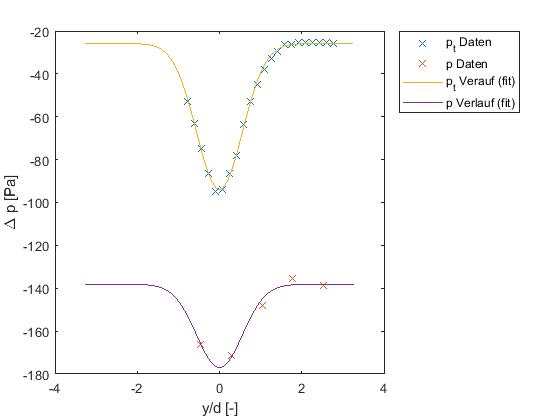
\includegraphics[width=0.75\textwidth]{Druckverlaeufe_Nachlauf_ohneAkt.jpg}
	\caption{ $\Delta P$ \"uber y/d ohne Aktuierung }
	\label{fig:Deltap-y/d_ohne_Aktuation}
\end{figure}

\section{Konstellation 1: Reine Rotation (KK)}
\label{s:ReineRotation}

In  \abb{fig:Cw-n_Rein_Konf+2} sind die Widerstandsbeiwerte von beiden Wellenpaaren bei verschiedenen Wellendrehzahlen zu sehen.
Die nat\"urliche Abl\"osefrequenz wird bei einer Drehzahl von 1938 1/min  erreicht. F\"ur eine gute Vergleichbarkeit wird der Bereich vor und insbesondere nach dieser Drehzahl, sowohl bei den glatten als auch bei den gezahnten Wellen, genauer und hochaufl\"osender Untersucht.
Abgesehen davon, dass die Konfiguration mit den ovalen bzw. gezahnten Wellen, in allen Drehzahlbereichen einen geringeren $C_{w}$-Wert im Vergleich zur Basiskonfiguration aufweisen, ist das Verhalten der beiden Kurven jedoch unterschiedlich.
\begin{figure}[h]
	\centering
	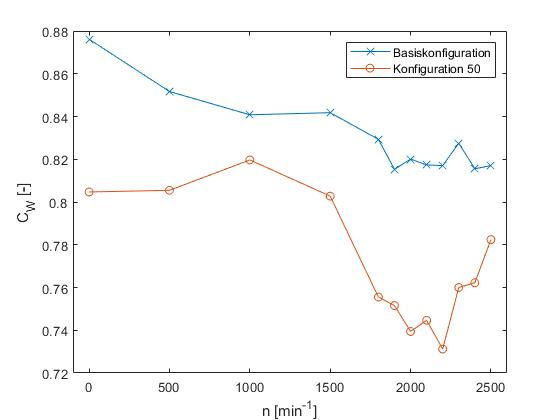
\includegraphics[width=0.5\textwidth]{Cw_ueber_n_ohneAB_beideKonf.jpg}
	\caption{ $C_{w}$-n reine Rotation beide Wellenpaare }
	\label{fig:Cw-n_Rein_Konf+2}
\end{figure}

W\"ahrend der $C_{w}$-Wert bei der Basiskonfiguration direkt nach der Impulsbeaufschlagung der Grenzschicht durch Rotation der Wellen, zu sinken anf\"angt, steigt der $C_{w}$-Wert der Konfiguration mit gezahnten Wellen bis zu einer Drehzahl von 1000 1/min. Erst ab einer Drehzahl von 1500 1/min, ist eine deutliche Widerstandsreduzierung zu erkennen. 
Anders als die Basiskonfiguration, bei der der minimale $C_{w}$-Wert im Bereich der erwarteten Abl\"osefrequenz erreicht wird, geschieht dies bei der Konfiguration 50 nach der Abl\"osefrequenz und zwar bei n= 2300. 
Beide Verl\"aufe steigen wieder, nachdem der niedrigste $C_{w}$-Wert erreicht wurde. Dennoch ist diese
Steigung mit den ovalen Wellen deutlich gr\"o\ss{}er.
Um von der Widerstandsreduzierung profitieren zu k\"onnen, muss noch genau verglichen werden, wie viel Leistung die jeweilige Konfiguration in Anspruch nimmt. Diese wird mit der kinetischen Leistung der Hauptstr\"omung genormt und als Leistungskoeffizient bezeichnet.

In \abb{fig:Cw-Cw0-CpowerM_reine} ist das $\Delta$ $C_{w}$-$C_{Power}$-Diagramm zu sehen. Es ist deutlich erkennbar, dass die ovalen Wellen, wesentlich mehr Energie ben\"otigen, um die Reibung zwischen der Teflonoberfl\"ache und dem Ausblaseschlitz zu \"uberwinden. Dazu kommt, dass die ovalen Wellen bei niedrigen Drehzahlen erst eine Widerstandssteigerung verursachen. 

Bei der Basiskonfiguration sinkt der $\Delta$ $C_{w}$-Wert, bereits bei geringer Energiezufuhr.  Nachdem der niedrigste Widerstandsbeiwert bei einer $C_{Power}$= 0,2 erreicht wurde f\"angt die Kurve an, lokal zu schwanken. Dies kommt durch die hohe lokale Drehzahlaufl\"osung im Bereich der Abl\"osefrequenz zustande. Laut Diagramm w\"urde sich nicht lohnen, die glatten Wellen mit einer h\"oheren Drehzahl als 1900  1/min zu drehen, da bei weiterer Energiezufuhr, keine Widerstandsreduzierung zu erkennen ist.
\begin{figure}[h]
	\centering
	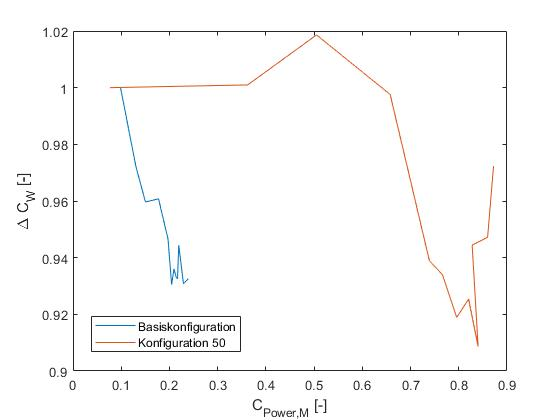
\includegraphics[width=0.5\textwidth]{DeltaCw_ueberC_PowerM_ohne_AB_beideKonf.jpg}
	\caption{ $C_{w}$/$C_{w0}$ \"uber $C_{Power,M}$ f\"ur reine Rotation  }
	\label{fig:Cw-Cw0-CpowerM_reine}
\end{figure}
Bei der Konfiguration mit den ovalen Wellen muss deutlich mehr Leistung aufgebracht werden, um eine Widerstandsreduzierung im Vergleich zu der Konfiguration ohne Aktuieren zu erhalten.  Erst ab einem $C_{Power}$ von ca. 0,65 wird ein $C_{w}$/$C_{w0}$ erreicht, der kleiner als 1 ist. 
Danach sinkt der $C_{w}$-Wert stark un erreicht den kleinsten $C_{w}$-Wert bei einem $C_{Power}$= 0,84. 
Der minimale $C_{w}$/$C_{w0}$ ist zwar kleiner als bei der Basiskonfiguration und somit die Widerstandsreduzierung gr\"o\ss{}er, jedoch muss deutlich mehr Leistung aufgebracht werden.
\begin{table}[h]
	\centering
	\begin{tabular}{lrr}
		\toprule
		 & kleinster  $C_{w}$/$C_{w0}$ & $C_{Power}$ beim kleinsten $C_{w}$/$C_{w0}$ \\
		\midrule
		Basiskonfiguration & 0.93 & 0.2\\
		Konfiguration 50 & 0.91 & 0.84\\
		\bottomrule
	\end{tabular}\\
	\caption{ minimale  $C_{w}$-Werte und die entsprechenden $C_{Power}$ }
	\label{tab:minimalCw-Cpower}
\end{table}
Der Tabelle 6.5 zu entnehmen, muss man die Leistung um 420\% steigern, um mit den ovalen Wellen einen um ca. 2\% geringeren $C_{w}$/$C_{w0}$ als die Basiskonfiguration zu bekommen.

%%%%%%%%%%%%%%%%%%%%%%%%%%%%%%%%%%%%%%%%%%%%%%%%%%%%%%%%%%%%%%%%%%%%%%%%%%%%%%%%%%%%%%%%%%%%%%%%%%%%%%%%%%%

\section{Konstellation 2: Reine Ausblasung (AK)}
\label{s:reineAusblasung}
In \abschn{s:reineAusblasung} wurde das Profilmodell mit den glatten Welle im Windkanal eingebaut.Es gab keine Rotation bei den Wellen und der Versuch wurde mit den glatten Wellen ohne Aktuation durchgef\"uhrt. Der Volumenstrom wurde so eingestellt, dass
die folgenden $C_{\mu}$  Werte erreicht werden. Es wurde $C_{w}$ mit diesen vier verschiedenen $C_{\mu}$ Werte gemessen.Die Ergbnisse sind wie folgt:
\begin{table}[H]
	\centering
	\begin{tabular}{lr}
		\toprule
		$C_{\mu}$ & $C_{w}$ \\
		\midrule
		0.00 & 0.876\\
		0.16 & 0.606\\
		0.32 & 0.477\\
		0.48 & 0.399\\
		0.69 & 0.331\\
		\bottomrule
	\end{tabular}
	\caption{$C_{w}$ und $C_{\mu}$ mit der glatten Welle ohne Aktuation }
	\label{tab:Cw-Cmu_Kon1}
\end{table}


Die \abb{fig:Cw-Cmu_Konf1} zeigt die Funktion von Widerstandsbeiwert \"uber Impulsbeiwert f\"ur die glatte welle ohne Atuation:
\begin{figure}[h]
	\centering
	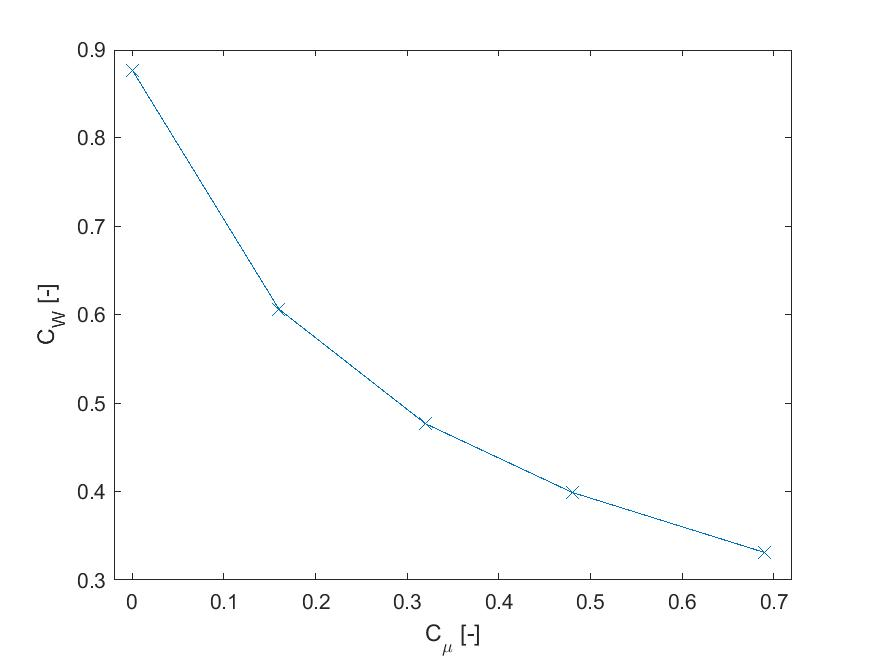
\includegraphics[width=0.5\textwidth]{Cw_ueber_Cmu_ohne_n.jpg}
	\caption{$C_{w}$  \"uber $C_{\mu}$ mit den glatten Wellen ohne Aktuation }
	\label{fig:Cw-Cmu_Konf1}
\end{figure}

Wie man im Diagramm betrachtet, ist es ein deutlicher Abfall von $C_{w}$ mit steigendem $C_{\mu}$.
F\"ur den Versuch mit den ovalen Wellen wurde $C_{\mu}$ Werte f\"ur die Verschiedenen Luftdr\"ucke berechnet. Unten sind die Auswertungen f\"ur $C_{w}$:
 
\begin{table}[h]
	\centering
	\begin{tabular}{lrr}
		\toprule
		Luftdruck [kPa] & $C_{\mu}$ & $C_{w}$ \\
		\midrule
		0 & 0.00 & 0.805\\
		1 & 0.06 & 0.610\\
		2 & 0.27 & 0.594\\
		3 & 0.42 & 0.577\\
		4 & 0.58 & 0.455\\
		\bottomrule
	\end{tabular}\\
	\caption{Luftdruck, $C_{w}$  und $C_{\mu}$ f\"ur die glatten und ovalen Wellen ohne Aktuation}
	\label{tab:Cw-Cmu_Konf1+2}
\end{table}

Die \abb{fig:Cw-Cmu_Konf1+2} zeigt den Verlauf $C_{w}$ \"uber $C_{\mu}$ f\"ur die beiden Konfigurationen:
\begin{figure}[h]
	\centering
	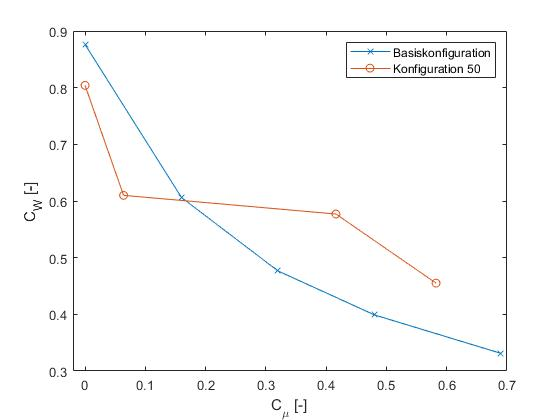
\includegraphics[width=0.5\textwidth]{Cw_ueber_Cmu_ohne_n_beideKonf.jpg}
	\caption{$C_{w}$  \"uber $C_{\mu}$ mit den glatten Wellen ohne Aktuation }
	\label{fig:Cw-Cmu_Konf1+2}
\end{figure}

Wie man im Diagramm sieht, f\"allt auch $C_{w}$  mit steigendem $C_{\mu}$  mit den ovalen Wellen ab.
\\
Im Vergleich mit den glatten Wellen sind die Widerstandsbeiwerte bei Impulskoeffizient im Bereich von 0 bis 0.16  in den ovalen Wellen niedriger als den glatten Wellen. Aber ab dem Punkt $C_{\mu}$= 0.16 sinkt der Widerstandsbeiwert der glatten Wellen st\"arker ab. Aus diesem Grund sind die glatten Wellen ohne Aktuation bei den gr\"o\ss{}eren Impulskoeffiziente zu empfehlen.

Dann werden die verschiedenen Widerstandsbeiwerte in Abh\"ungigkeit vom Leistungskoeffizient gemessen. Die Tabelle 6.3 ermittelt diese Werte f\"ur die Basiskonfiguration:
\begin{table}[h]
	\centering
	\begin{tabular}{lr}
		\toprule
		$C_{w}$/$C_{w0}$ & $C_{Power,Jet}$ \\
		\midrule
		1 & 0\\
		0.691 & 0.010\\
		0.544 & 0.283\\
		0.455 & 0.520\\
		0.378 & 0.896\\
		\bottomrule
	\end{tabular}
	\caption{$C_{w}$/$C_{w0}$ \"uber $C_{Power,Jet}$ f\"ur Basiskonfiguration }
	\label{tab:Cw/Cw0-CpJet_Kon1}
\end{table}

Und die Auswertungen f\"ur die Konfiguration mit den ovalen Wellen sind in der Tabelle 6.4:

\begin{table}[h]
	\centering
	\begin{tabular}{lr}
		\toprule
		$C_{w}$/$C_{w0}$ & $C_{Power,Jet}$ \\
		\midrule
		1 & 0\\
		0.748 & 0.149\\
		0.718 & 0.773\\
		0.566 & 1.90\\
		\bottomrule
	\end{tabular}
	\caption{$C_{w}$/$C_{w0}$ \"uber $C_{Power,Jet}$ f\"ur die ovalen Wellen }
	\label{tab:Cw/Cw0-CpJet_Kon2}
\end{table}

Die \abb{fig:Cw/Cw0-CpJet_Konf1+2} zeigt den Verlauf $C_{w}$/$C_{w0}$ \"uber $C_{Power,Jet}$  f\"ur die beiden Konfigurationen:
\begin{figure}[h]
	\centering
	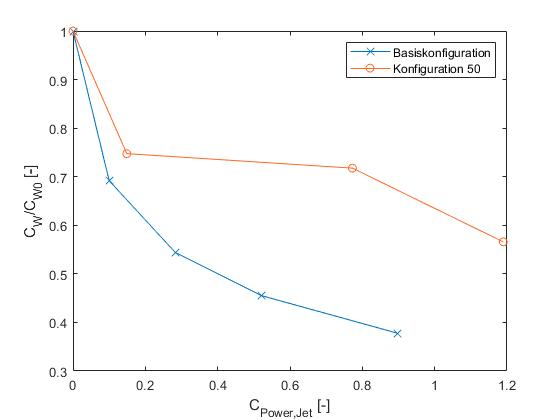
\includegraphics[width=0.5\textwidth]{CwC0_ueber_CPowerJ_ohne_n_beideKonf.jpg}
	\caption{$C_{w}$/$C_{w0}$  \"uber $C_{Power,Jet}$ f\"r die beiden Konfigurationen}
	\label{fig:Cw/Cw0-CpJet_Konf1+2}
\end{figure}

Wie aus dem Diagramm ersichtlich ist, wird mehr Leistung ben\"otigt, um einen niedriegen Wiederstansbeiwert $C_{w}$  zu erreichen. Mit den ovalen Wellen wird mehr Leistung als den glatten Wellen ben\"otigt, um die gleiche Widerstandsreduzierung zu erzielen. Deswegen weist die Konfiguration mit den glatten Wellen in diesem Fall bessere Ergebnisse auf.
\newpage

\section{Konstellation 3: Kombinierte Aktuation (KK)}
\label{s:kombinierteAkt}
Nun wird bei beiden Konfigurationen, sowohl durch die Walzen als auch durch die Ausblasung aktuiert.\\

Die in \kap{s:reineAusblasung} verwendeten $C_{\mu}$-Werte f"ur die Konfiguration mit ovalen Wellen beziehen sich auf eine Wellenstellung, bei der der Spalt maximal ge"offnet ist, die Spalth"ohe also ca. 0,3\,mm betr"agt. Diese Position kann als einzige ge"offnete Wellenposition definiert eingestellt werden und dient der besseren Vergleichbarkeit mit der Basiskonfiguration. Wenn die Rotation hinzugenommen wird, "andert sich das $C_{\mu}$ allerdings und muss nach \glg{eq:momentum-coeff-oscill-final} berechnet werden. Die mit dem urspr"unglichen Impulskoeffizienten korrespondierenden neuen $C_{\mu}$-Werte sind in \tab{tab:Cmu Korrektur} festgehalten.

\begin{table}[H]
	\centering
	\begin{tabular}{lr}
		\toprule
		$C_{\mu}$ (reine Ausblasung) & $C_{\mu}$ (kombinierte Aktuation)\\
		\midrule
		0 & 0\\
		0,064 & 0,097\\
		0,27 & 0,231\\
		0,416 & 0,29\\
		0,582 & 0,327\\
		\bottomrule
	\end{tabular}
	\caption{Korrespondierende $C_{\mu}$-Werte f"ur reine Ausblasung und kombinierter Aktuation bei Konfiguration 50}
	\label{tab:Cmu Korrektur}
\end{table}


F"ur die Betrachtungen und Abbildungen wird aus "Ubersichtlichkeitsgr"unden das urspr"ungliche $C_{\mu}$ verwendet. Dieser Zusammenhang erschwert die Interpretation allerdings und muss stets im Hinterkopf behalten werden.

Die Vergleichbarkeit mit der Basiskonfiguration ist hier zus"atzlich dadurch eingeschr"ankt, dass nur bis zu mittleren Plenumsdr"ucken von 4\,kPa gemessen wurde und die Impulskoeffizienten f"ur diese Konfiguration nicht die, der Basiskonfiguration erreichen.\\
"Hohere Dr"ucke k"onnen gleichwohl nicht mitbetrachtet werden, da bei einem d"unnen verbleibenden Spalt die Dr"ucke deutlich "uber 9\,kPa liege, was wiederum in Jetgeschwindigkeiten oberhalb $Ma =$ $\frac{1}{3}$ m"undet. Die Annahme der inkompressiblen Jetstr"omung kann dann nicht mehr getroffen werden.

In \abb{fig:Cw/n bei Cmu RK} ist $C_{W}$ "uber n bei verschiedenen $C_{\mu}$ f"ur die Basiskonfiguration dargestellt.

\begin{figure}[h]
	\centering
	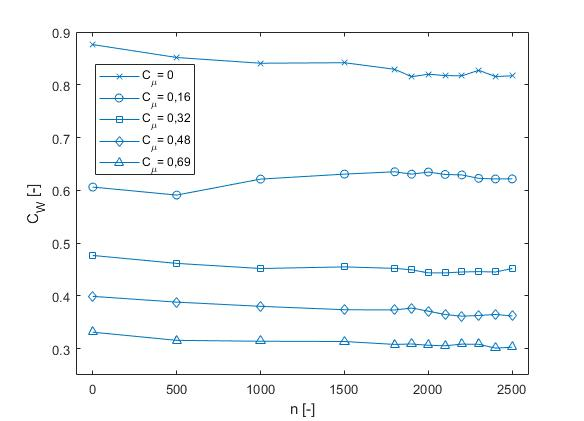
\includegraphics[width=0.5\textwidth]{Cw_ueber_n_fuer_verschiedeneCmu_RK.jpg}
	\caption{$C_{w}$ "uber $n$ bei verschiedenen $C_{\mu}$ f"ur die Basiskonfiguration}
	\label{fig:Cw/n bei Cmu RK}
\end{figure}

Au\ss{}er bei $C_{\mu}= 0,16$ sind alle anderen Verl"aufe in Abh"angigkeit von der Drehzahl "ahnlich.
Sie sinken mit einer "ahnlichen Rate bis zum Bereich der nat"urlichen Abl"osefrequenz und schwanken leicht wachsend danach.\\Mit einem $C_{\mu}= 0,16$ wird der $C_{W}$-Verlauf bis auf $n= 500$, wo der Widerstand minimal reduziert wird, immer oberhalb des $C_{W}$ der reinen Ausblasung gehalten. In diesem Fall bedeutet eine zus"atzliche Rotation mehr Energie und Aufwand, und steigert den Widerstandsbeiwert.

Bei der Betrachtung der $C_{W}-n$-Verl"aufe in Abh"angigkeit von den Impulskoeffizienten ist ersichtlich, dass diese mit steigendem $C_{\mu}$ degressiv sinken und eine Ausblasung unabh"angig von der Drehzahl einen gro\ss{}en ANteil an der Widerstandsreduzierung hat.

Bei den ovalen Wellen ist die Abh"angigkeit der $C_{W}$-Werte von den Impulskoeffizienten "ahnlich wie bei der Basiskonfiguration (\abb{fig:Cw/n bei Cmu 50}).
\begin{figure}[h]
	\centering
	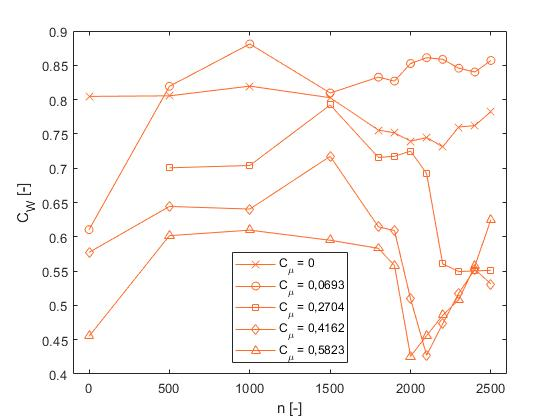
\includegraphics[width=0.5\textwidth]{Cw_ueber_n_fuer_verschiedeneCmu_50.jpg}
	\caption{$C_{w}$ "uber $n$ bei verschiedenen $C_{\mu}$ f"ur die Konfiguration 50}
	\label{fig:Cw/n bei Cmu 50}
\end{figure}

Die zus"atzliche Rotation der Walzen ist aber nur bei bestimmten $C_{\mu}$ und Drehzahlen widerstandsreduzierend. Bei allen $C_{\mu}$ wird der $C_{W}$ bei Beginn der Rotation erh"oht, bis er wieder im Bereich der Abl"osefrequenz einbricht. Allerdings ist Sensibilit"at bei h"oheren $C_{\mu}$ in diesem Frequenzbereich sehr hoch, sodass der Widerstand deutlich erh"oht wird, wenn die optimale Drehzahl nicht getroffen wird.

In der \abb{fig:CwCwref/n Cmu RK} sind die mit dem jeweiligen $C_{ref}$ normierten $C_{W}$-Werte der Basiskonfiguration, bei verschiedenen $C_{\mu}$ zu sehen.
Als jeweiliges $C_{ref}$ dient hierbei der $C_{W}$-Wert des entsprechenden $C_{\mu}$s ohne Rotation.


\begin{figure}[h]
	\centering
	\begin{subfigure}[c]{0.45\textwidth}		
		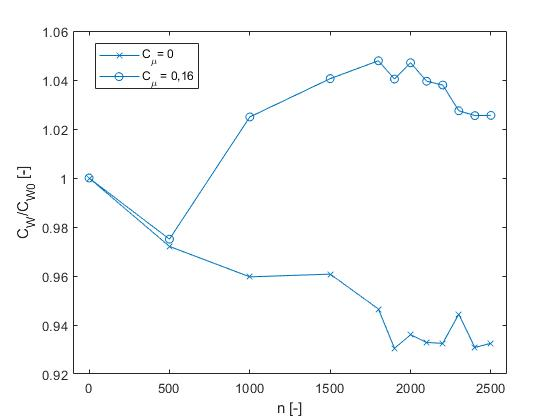
\includegraphics[width=1\textwidth]{CwCw0_ueber_n_fuer_2Cmus_RK.jpg}
		%\subcaption{}
	\end{subfigure}
	\begin{subfigure}[c]{0.45\textwidth}
		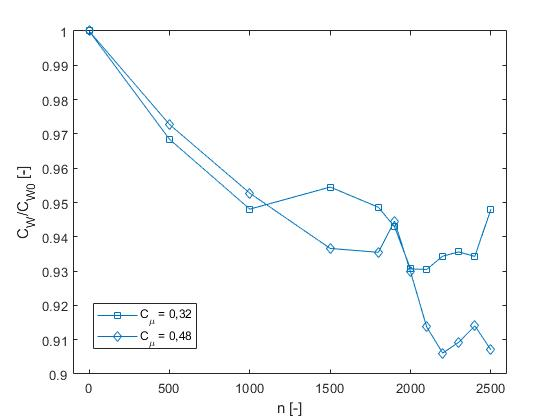
\includegraphics[width=1\textwidth]{CwCw0_ueber_n_fuer_Cmu3und4_RK.jpg}
		%\subcaption{}
	\end{subfigure}
	\begin{subfigure}[c]{0.45\textwidth}
		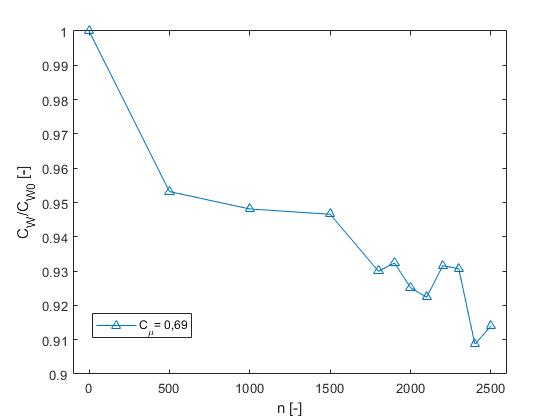
\includegraphics[width=1\textwidth]{CwCw0_ueber_n_fuer_Cmu5_RK.jpg}
		%\subcaption{}
	\end{subfigure}
	\caption{$C_{W}/C_{Wref}$ "uber n bei verschiedenen $C_{\mu}$ f"ur die Basiskonfiguration}
	\label{fig:CwCwref/n Cmu RK}
\end{figure}

In der \abb{fig:CwCwref/n Cmu 50} sind die mit dem jeweiligen $C_{ref}$ normierten $C_{W}$-Werte der Konfiguration 50, bei verschiedenen $C_{\mu}$ zu sehen.
Als jeweiliges $C_{ref}$ dient hierbei der $C_{W}$-Wert des entsprechenden $C_{\mu}s$ ohne Rotation.

\begin{figure}[h]
	\centering
	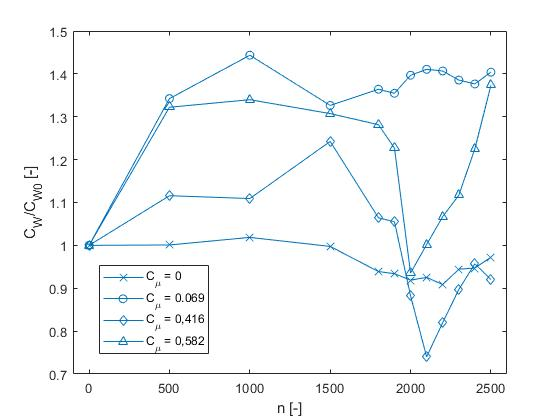
\includegraphics[width=0.5\textwidth]{CwC0_ueber_n_fuer_Cmus_50.jpg}
	\caption{$C_{W}/C_{Wref}$ "uber n bei verschiedenen $C_{\mu}$ f"ur die Konfiguration 50}
	\label{fig:CwCwref/n Cmu 50}
\end{figure}

In den \abb{fig:PR} sind die Leistungsraten beider Konfigurationen bei verschiedenen Impulskoeffizienten und Drehzahlen ersichtlich.\\
Ein $PR= 1$ bedeutet, dass man so viel Energie mit der Widerstandsreduzierung erspart hat, wie man Energie f"ur dieselbe eingesetzt hat. In so einem Fall wird man sich in der Realit"at gegen diese widerstandsreduzierenden Ma\ss{}nahmen entscheiden, da diese nur erh"ohten Zeitaufwand, h"ohere Kosten und Reparaturanf"allifgkeit, ein gesteigertes Gewicht und weitere negative Nebenwirkungen zur Folge haben.

\begin{figure}[h]
	\centering
	\begin{subfigure}[c]{0.45\textwidth}		
		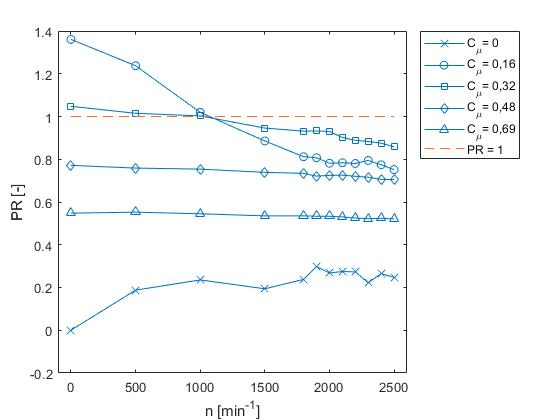
\includegraphics[width=1\textwidth]{PR_uber_n_fuer_Cmu_RK.jpg}
		\subcaption{$PR$ f"ur die Basiskonfiguration}
		\label{fig:PR RK}
	\end{subfigure}
	\begin{subfigure}[c]{0.45\textwidth}
		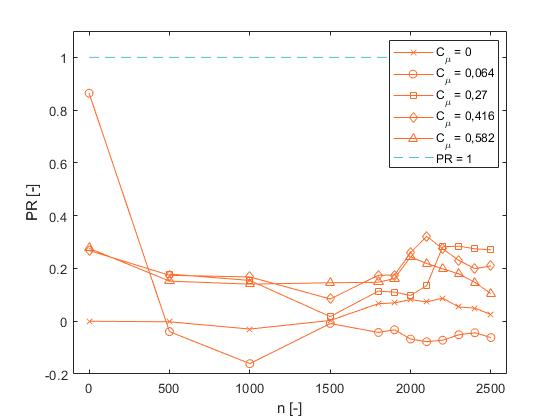
\includegraphics[width=1\textwidth]{PR_ueber_n_fuer_Cmu_50.jpg}
		\subcaption{$PR$ f"ur die Konfiguration 50}
		\label{fig:PR 50}
	\end{subfigure}
		\caption{$PR$ "uber $n$ bei verschiedenen $C_{\mu}$ f"ur beide Konfigurationen}
	\label{fig:PR}
\end{figure}

Es wird deutlich, dass die Konfiguration 50 bei keiner Drehzahl und keinem $C_{\mu}$ den Wert 1 erreicht, oder "uberschreitet. Der wichtigste zu nennende Grund daf"ur ist die gro\ss{}e Reibung zwischen der Teflonschicht und dem Ausblaseschlitz, die durch die Motoren "uberwunden werden muss. Diese aufzubringende Kraft ist unter anderem so gro\ss{}, da man gewisse Vorspannkr"afte aufbringen musste, um den vordefinierten Signalverlauf sicherzustellen.

Die Basiskonfiguration erreicht im Vergleich zu der gezahnten Konfiguration eine deutlich h"ohere Effektivit"at, auch wenn nicht immer vorteilhaft, da gerade nur bei zwei $C_{\mu}$s und einer Drehzahl bis ca. $1000$\,$min^{-1}$ Leistung erspart werden kann. Allerdings wird deutlich, dass die Bestwerte bei reiner Ausblasung erreicht werden. Die Widerstandsreduzierung der rotierenden Walzen verursacht einen gro\ss{}en energetischen Aufwand, sodass die Leistungsersparnis trotz einer Widerstandsreduzierung kleiner wird oder sogar in Leistungsverlust umgewandelt wird.